%\begin{figure}[!htbp]
%    \centering
%    \caption{}
%    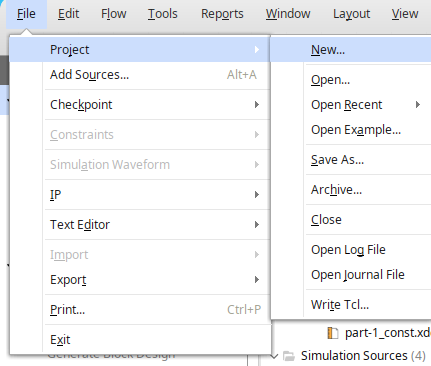
\includegraphics[width=0.5\textwidth]{figure_3_1.png}
%    \label{Figure 3.1}
%\end{figure}\newline

%\begin{center}
%    Truth Table 1: AND Gate Waveform
%    \begin{displaymath}
%    \begin{array}{|c c|c|}
%    In1 & In2 & In1 \land In2\\
%    \hline
%    F & F & F\\
%    F & T & F\\
%    T & F & F\\
%    T & T & T\\
%    \end{array}
%    \end{displaymath}
%\end{center}

\documentclass{article}
\usepackage{graphicx} % Required for inserting images
\usepackage{varwidth}
\usepackage{listings}
\usepackage{xcolor}

\title{Experiment 2 Lab Report \\ \large EEE3342C - 00012}
\author{Yousef Awad}
\date{January 2025}
\setcounter{secnumdepth}{0}

\lstdefinestyle{Verilog}{
  language=Verilog,
  basicstyle=\ttfamily\small,
  keywordstyle=\color{blue}\bfseries,
  commentstyle=\color{gray},
  stringstyle=\color{purple},
  numbers=left,
  numberstyle=\tiny,
  stepnumber=1,
  numbersep=5pt,
  tabsize=2,
  breaklines=true,
  captionpos=b,
  frame=single
}

\begin{document}

\maketitle
\tableofcontents
\newpage

\section{Equipment}
For this experiment a computer running Linux 6.12.13 was used alongside the Xilinx Vivado 2024.2 software, alongside an FPGA board, the BASYS 3 development board. The board specifically only used to ensure the simulation by the Vivado software was accurate in the real world, as well as to verify the simulation software wasn't incorrect.
\section{Objective}
\section{Part 1: Half/Full Adder}
\subsection{Half Adder}
The circuit given for this part was the following:
$$ \neg[(A \land B) \lor \neg (C \lor D)] $$
Of which has the following given schematic:
\begin{figure}[!htbp]
    \centering
    \caption{Schematic for Half Adder}
    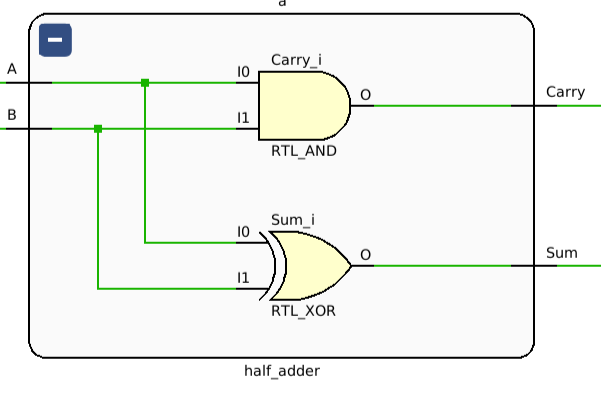
\includegraphics[width=0.5\textwidth]{part-1-half-schem.png}
    \label{Half Adder Schematic}
\end{figure}
And when compiled into a truth table with the inputs of A, B, and an output of Carry, would be the following:
\begin{center}
    Truth Table for Half Adder
    \begin{displaymath}
    \begin{array}{|c c|c c|}
      A & B & Output & Carry\\
    \hline
    F & F & F & F \\
    F & T & T & F \\
    T & F & T & F \\
    T & T & F & T \\
    \end{array}
    \end{displaymath}
\end{center}
And when written up in verilog, has the following text:
\begin{figure}[!htbp]
    \centering
    \begin{verbatim}
    module half_adder(
          input A, B,
          output Sum, Carry
      );
      
      assign Sum = A ^ B;
      assign Carry = A & B;
      
    endmodule
    \end{verbatim}
\end{figure}
And when tested, used the following testbench, after reading through part 1 of the experiment manual:
\begin{lstlisting}[caption={test}, label={label}, style=Verilog]
module testbench();
    parameter numin = 2;
    integer i;
    reg[numin - 1:0] count;
    
    reg a, b;
    wire carry, sum;
    
    half_adder UUT(.A(a), .B(b), .Carry(carry), .Sum(sum));

    
    initial begin
        count = 0;
        for ( i = 0; i < 2**numin; i = i + 1 ) begin
            assign a = count[1];
            assign b = count[0];
            
            count = count + 1;
            #10;
        end
    end
    
endmodule
\end{lstlisting}
And, when simulated to confirm the truth table above to be true or false, it gave out the following waveform:
\begin{figure}[!htbp]
    \centering
    \caption{Waveform for the Half-Adder}
    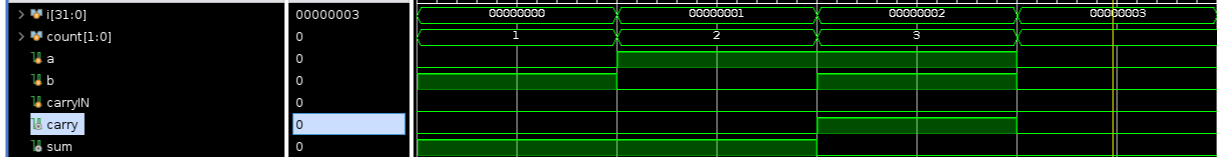
\includegraphics[width=1\textwidth]{part-1-half-waveform.png}
    \label{Figure 2}
\end{figure}
Of which perfectly shows that the truth table compiled above for the circuit is accurately shown in the simulation on Vivado. To ensure, even further, I then pushed the bitstream generated onto the BASYS board to manually enter and double check the simulation/truth table proper by flicking every possible combination.
\newpage

\subsection{Full Adder}
The circuit schematic given for this part was the following:
\begin{figure}[!htbp]
    \centering
    \caption{Schematic for Full Adder}
    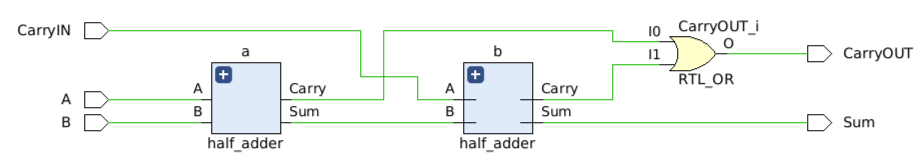
\includegraphics[width=0.5\textwidth]{part-1-full-schem.png}
    \label{Full Adder Schematic}
\end{figure}
And when written up in verilog, has the following text:
\begin{lstlisting}[caption={test}, label={label}, style=Verilog]
module full_adder(
        input A, B, CarryIN,
        output Sum, CarryOUT
    );
    
    wire carry1, carry2, sum1;
    
    half_adder a(.A(A), .B(B), .Carry(carry1), .Sum(sum1));
    half_adder b(.A(CarryIN), .B(sum1), .Sum(Sum), .Carry(carry2));
    
    assign CarryOUT = carry1 | carry2; 
    
endmodule
\end{lstlisting}
And when tested, used the following testbench, after reading through part 1 of the experiment manual:
\begin{lstlisting}[caption={test}, label={label}, style=Verilog]
module testbench();
    parameter numin = 2;
    integer i;
    reg[numin - 1:0] count;
    
    reg a, b, carryIN;
    wire carry, sum;
    
    full_adder UUT(.A(a), .B(b), .CarryIN(carryIN), .CarryOUT(carry), .Sum(sum));

    
    initial begin
        count = 0;
        for ( i = 0; i < 2**numin; i = i + 1 ) begin
            assign a = count[1];
            assign b = count[0];
            assign carryIN = 0;
            
            count = count + 1;
            #10;
        end
    end
    
endmodule
\end{lstlisting}
And, when simulated, it gave out the following correct waveform:
\begin{figure}[!htbp]
    \centering
    \caption{Waveform for the Half-Adder}
    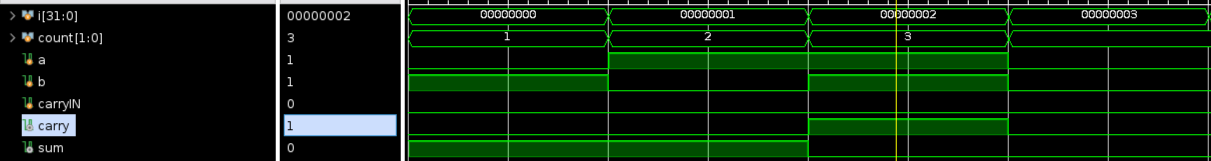
\includegraphics[width=1\textwidth]{part-1-full-waveform.png}
    \label{Figure 2}
\end{figure}
To ensure, even further past the given truth table in lab report, I then pushed the bitstream generated onto the BASYS board to manually enter and double check the simulation proper by flicking every possible combination.
\newpage


\section{Part 1: 8-Bit Ripple Carry Adder}
The schematic was designed as following:
\begin{figure}[!htbp]
    \centering
    \caption{Schematic for 8 Bit Ripple Carry Adder}
    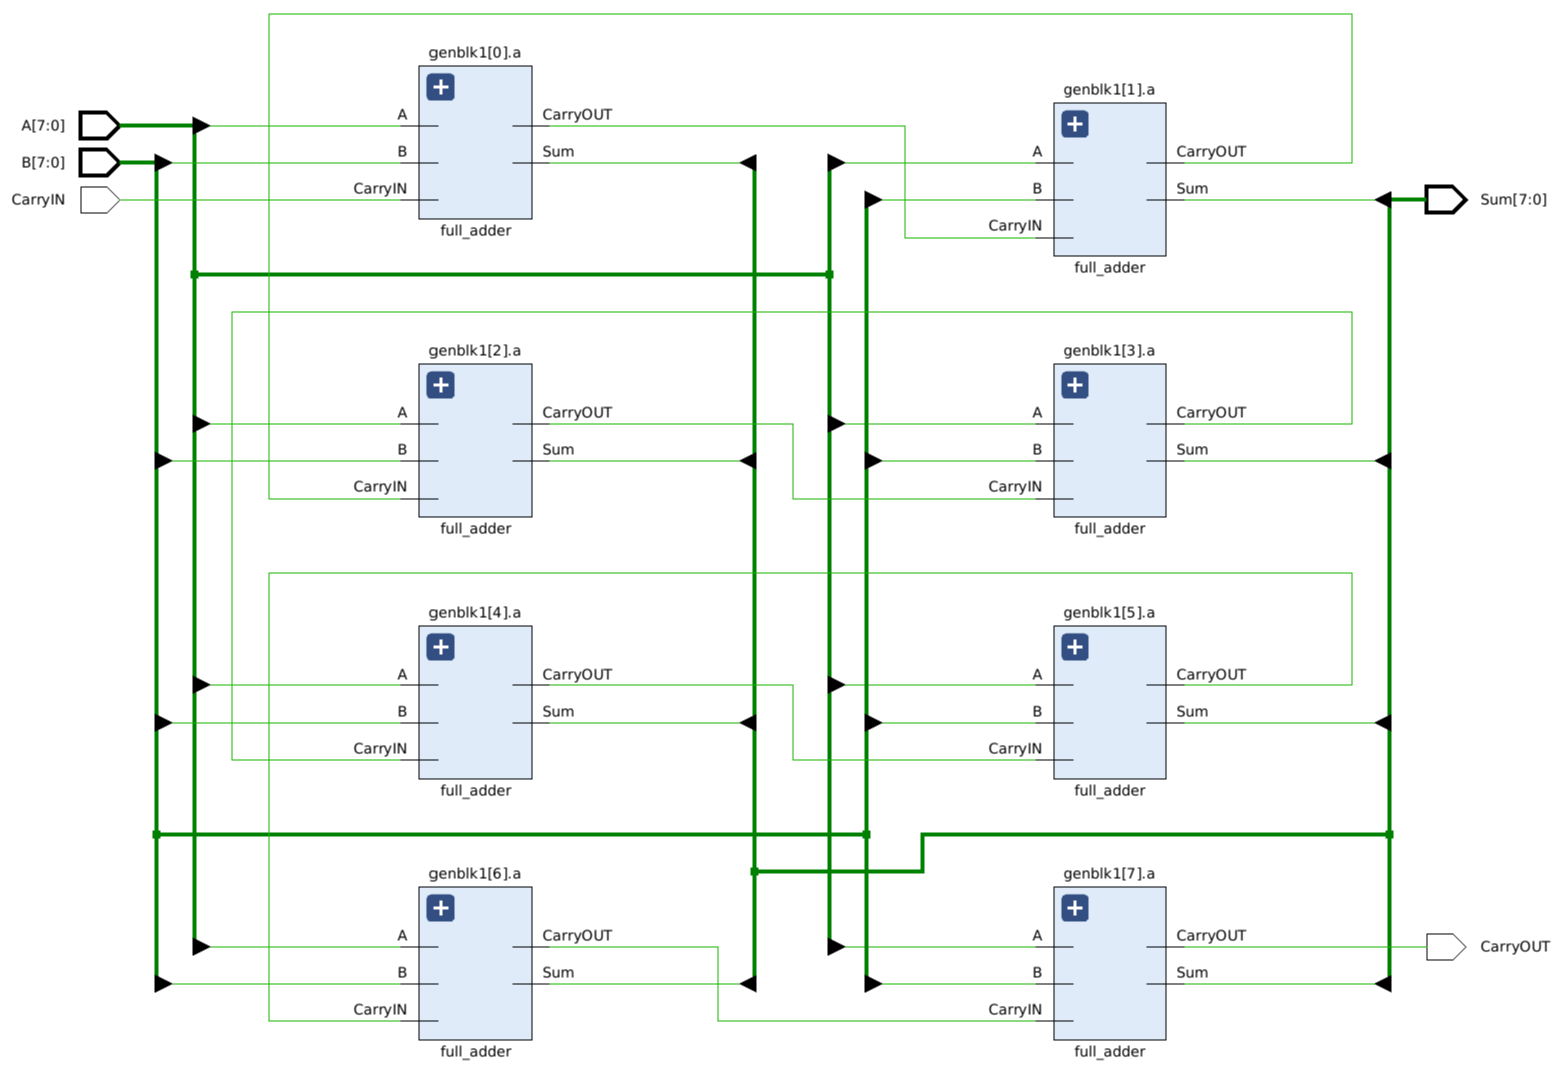
\includegraphics[width=0.5\textwidth]{part-2-schem.png}
    \label{8 Bit Ripple Carry Schematic}
\end{figure}
And when written up in verilog, has the following text:
\begin{lstlisting}[caption={test}, label={label}, style=Verilog]
module eight_bit_ripple_adder(
        input[7:0] A, B, 
        input CarryIN,
        output[7:0] Sum, 
        output CarryOUT
    );
    
    wire[8:0] carry;
    
    assign carry[0] = CarryIN;
    
    genvar i;
    
    generate
        for ( i = 0; i < 8; i = i + 1 ) begin
            full_adder a(.A(A[i]), .B(B[i]), .CarryIN(carry[i]), .CarryOUT(carry[i + 1]), .Sum(Sum[i]));
        end
    endgenerate
    
    assign CarryOUT = carry[8];
    
endmodule
\end{lstlisting}
And when tested, used the following testbench, after reading through part 1 of the experiment manual:
\begin{lstlisting}[caption={test}, label={label}, style=Verilog]
module testbench_part2();
    parameter numin = 8;
    
    reg[numin - 1:0] a, b;
    reg carryIN;
    wire[numin - 1:0] sum;
    wire carryOUT;
    
    eight_bit_ripple_adder UUT(.A(a), .B(b), .CarryIN(carryIN), .CarryOUT(carryOUT), .Sum(sum));
    
    initial begin
        assign a = 8'b11001011;
        assign b = 8'b10101010;
        assign carryIN = 0;
        #10;
        assign carryIN = 1;
        #10
        assign a = 0;
        assign b = 0;
        assign carryIN = 0;
    end
    
endmodule
\end{lstlisting}
And, when simulated to confirm the addition of 170 and 203 (assuming it is unsigned) above to be 0x75 Carry 1 as it overflows and switches sign, it gave out the following waveform:
\begin{figure}[!htbp]
    \centering
    \caption{Waveform for Addition of 0x170 and 0x203}
    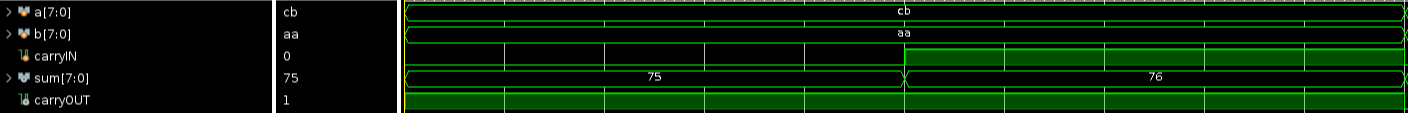
\includegraphics[width=1\textwidth]{part-2-waveform.png}
    \label{Waveform for Addition of 170 and 203}
\end{figure}
Of which perfectly shows the correct result to be 0x75 or 0x76 of which is in binary either 01001011 or 01001100 and in decimal is 117, depending on the carry in value with a carry out of 1 meaning it overflowed.
\newpage


\section{Conclusion}



\end{document}
